\documentclass{beamer}

%============= BASE PACKAGES =============%
\usepackage[english]{babel}
\usepackage{amsfonts,amsmath,oldgerm}
\usepackage{listings}
\usepackage{colortbl}
\usepackage{listings}
\usepackage{xcolor}
\usepackage{minted}
\definecolor{CodeBG}{rgb}{0.9,0.9,0.95}

%== fancy packages
\usepackage{julialogo}
\usepackage{emoji}

%============= BIBLIOGRAPHY =============%
\usepackage{csquotes} % babel and biblatex
\usepackage[citestyle=reading,bibstyle=authortitle]{biblatex}
\addbibresource{biblio.bib}


%============= images =============%
\usepackage{multimedia}
\usepackage{graphbox}
\graphicspath{{./figures/}}


%============= TABLES =============%
\usepackage{makecell}


%============= BEAMER =============%
\usetheme[
	progressbar=frametitle,
]{metropolis}
%=== footline
\newlength\barwidth
\setlength\barwidth{24pt} % width of bars set here
\setbeamertemplate{footline}{%
    \begin{beamercolorbox}[wd=\paperwidth,sep=2pt]{mycol}%
    \kern10pt
    
\includegraphics[align=c, height=10pt]{
        logo_imcce_couleur.png}%
    \hfill%
    \insertshortauthor{} -- AstroCalcul%
    \hfill\hfill%
    {\insertframenumber/\inserttotalframenumber}%
    \end{beamercolorbox}%
}
\setbeamerfont{footline}{size=\tiny, series=\sc}
\setbeamercolor{mycol}{
	% fg=gray,
	%bg=mDarkTeal!30
}
%=== block
\setbeamercolor{block body}{bg=mDarkTeal!30}
\setbeamercolor{block title}{bg=mDarkTeal,fg=black!2}
%=== misc
\usefonttheme[onlymath]{serif}
\setbeamertemplate{caption}[numbered]
\usepackage{appendixnumberbeamer}


%============= MISC =============%
%=== danger
\newcommand*{\TakeFourierOrnament}[1]{{%
\fontencoding{U}\fontfamily{futs}\selectfont\char#1}}
\newcommand*{\danger}{\TakeFourierOrnament{66}}
%=== newline in hyperlinks
\pdfstringdefDisableCommands{%
  \def\\{}%
}
%=== custom commands
\newcommand{\real}{\mathbb{R}}
\newcommand{\emphcell}{\cellcolor{mDarkTeal}}

%============= TITLE =============%
\title{A brief introduction to Julia}
% \subtitle{}
\author[A. Prieur]{Alexandre Prieur}
\institute{%
\raisebox{-.5\baselineskip}{
\includegraphics[width=3cm]{logo_imcce_couleur.png}}%
}
\date{AstroCalcul Juin 2024}


\begin{document}
\setemojifont{TwemojiMozilla}

\maketitle


\section{Introduction}

\begin{frame}
    \frametitle{What is Julia?}
    \begin{displayquote}
        \julia is a high-level, high-performance dynamic language for technical computing.
    \end{displayquote}
\end{frame}

\begin{frame}[fragile]
    \frametitle{What is Julia?}
    
\begin{minted}[breaklines,escapeinside=<>,mathescape=true, linenos, numbersep=3pt, gobble=0, frame=lines, fontsize=\small, framesep=2mm,
    bgcolor=CodeBG]{julia}
α = 2π
for i in 1:2
    if exp(i * α * im) ≈ 1
        print("Yey!")
    else
        print("Oh no...")
    end
end
\end{minted}
% # Or you can do
% exp(α*im) ≈ 1 ? "Yey!" : "Oh no..." |> print #probably remove
\end{frame}

\begin{frame}
    \frametitle{What is Julia?}
    \begin{displayquote}
        \julia is a \alert<2>{high-level}, \alert<3>{high-performance} \alert<4>{dynamic} language for technical computing.
    \end{displayquote}
    \begin{itemize}
        \item<2-> Easy to learn and use
        \item<3-> Fast code
        \item<4-> Compiled just-in-time
    \end{itemize}
    % \begin{columns}
    %     \column{0.35\textwidth}
    %     
\includegraphics[width=\textwidth]{logo_julia.png}
    %     \column{0.6\textwidth}
    % \end{columns}
\end{frame}

\begin{frame}
    \frametitle{Some dates}
    \begin{itemize}
        \item 2012: first release
        \item 2018: 1.0 release
        \item Current: 1.10.4
    \end{itemize}
    \pause
    \vspace{10pt}
    \tiny
    \begin{table}[htbp]
        \centering
        \begin{tabular}{|r|c|c|c|c|c|c|c|c|c|c|c|c|}
            \hline
            Year & Jan & Feb & Mar & Apr & May & Jun & Jul & Aug & Sep & Oct & Nov & Dec \\ \hline
            2018 & & & & & & & & 1.0 & & & & \\ \hline
            2019 & 1.1 & & & & & & & 1.2 & & & 1.3 & \\ \hline
            2020 & & &  1.4 & & & & & 1.5 & & & & \\ \hline
            2021 & & & & & {\bf 1.6} & & & & & & 1.7 & \\ \hline
            2022 & & & & & & & & 1.8 & & & & \\ \hline
            2023 & & & & & {\bf 1.9} & & & & & & & 1.10 \\ \hline
        \end{tabular}
        \caption{Julia minor releases}
        \label{tab:julia_releases}
    \end{table}

\end{frame}


\section{[Interactive] Diving in the code}

\begin{frame}[fragile]
    \frametitle{TO DO in the interactive session}
    \begin{itemize}
        \item Installation
    \begin{minted}[breaklines,escapeinside=<>,mathescape=true, numbersep=3pt, gobble=0, frame=single, fontsize=\tiny, framesep=2mm]{bash}
    curl -fsSL https://install.julialang.org | sh
    \end{minted}
        \pause
        \item Basic manip
        \item Packages and environments
        \item REPL modes: code, package, help, terminal
        \item Quick look at Pluto, VS Code
        \item Showcase of JIT
    \end{itemize}
    Prime spiral: \small{\url{https://www.3blue1brown.com/lessons/prime-spirals}}
\end{frame}

\section{Capacities of Julia}

% \begin{frame}
%     \frametitle{Julia's strong points}
%     \begin{itemize}
%         \alert<1>{\item Ease of use \textit{and} performance}
%         \begin{itemize}
%             \item no
%         \end{itemize}
%         \pause
%         \alert<2>{\item Eliminates points of friction}
%         \begin{itemize}
%             \item \texttt{juliaup}, \texttt{Pkg.jl}
%             \item Unicode support, clear syntax
%         \end{itemize}
%         \pause
%         \alert<3>{\item Community}
%         \begin{itemize}
%             \item Welcoming online discourse
%             \item Available libraries
%         \end{itemize}
%         \pause
%         \alert<4>{\item Extensibility}
%         \begin{itemize}
%             \item Code is extensible by design
%             \item Developing a package is easy (pkg creation, Julia written in Julia)
%         \end{itemize}
%         \pause
%         \alert<5>{\item Reproducibility}
%         \begin{itemize}
%             \item Easy to install/update packages, manage environments\dots
%             \item Readability
%         \end{itemize}
%     \end{itemize}
% \end{frame}

% https://github.com/Datseris/whyjulia-manifesto?tab=readme-ov-file
% https://xkcd.com/1987/

\begin{frame}
    \frametitle{Strong points -- Easy and fast}
    \begin{table}[htbp]
        \centering
\begin{tabular}{c|c|c}
    & Coding & Execution \\ \hline
    Python, R, \dots 
        & \textcolor{green}{\bf Fast} \cellcolor{lightgray!50}
        & \textcolor{red}{\bf Slow}   \cellcolor{lightgray!50}
        \\ \hline
    C, FORTRAN, \dots
        & \textcolor{red}{\bf Slow}   \cellcolor{lightgray!50}
        & \textcolor{green}{\bf Fast} \cellcolor{lightgray!50}
    \only<2->{\\ \hline Julia*
        & \textcolor{green}{\bf Fast} \cellcolor{lightgray!50}
        & \textcolor{green}{\bf Fast} \cellcolor{lightgray!50}}
\end{tabular}
        \caption{The two language problem}
        \label{tab:two_language_pb}
    \end{table}

    \pause \pause
    \vspace{10pt}
    *\small{Although it creates the 1.5 language problem}
\end{frame}

\begin{frame}
    \frametitle{Strong points -- Easy and fast}
    \begin{figure}[htbp]
        \centering
        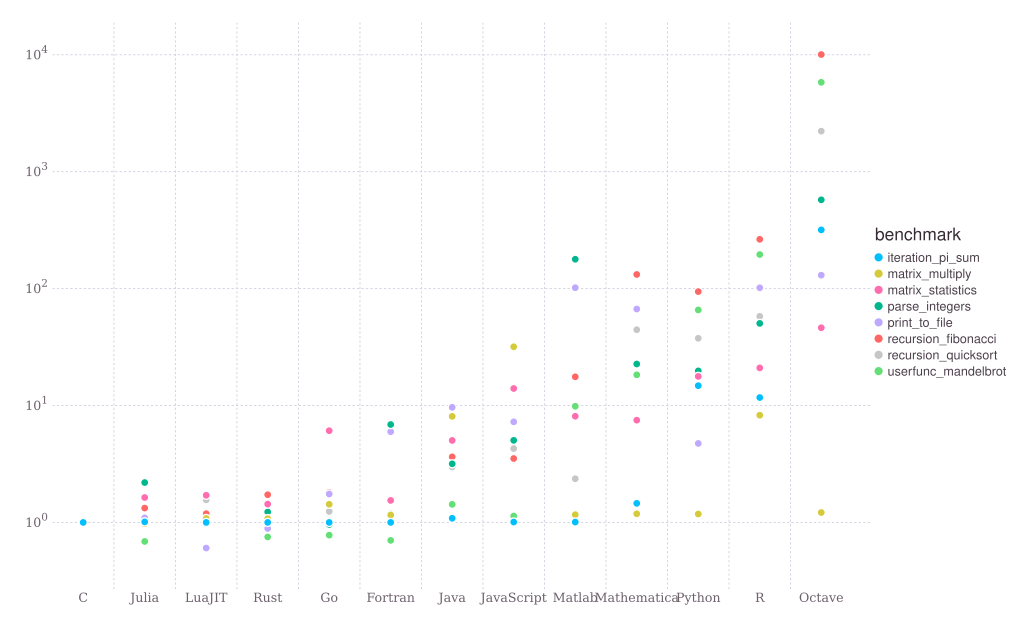
\includegraphics[width=0.8\textwidth]{benchmarks.png}
        %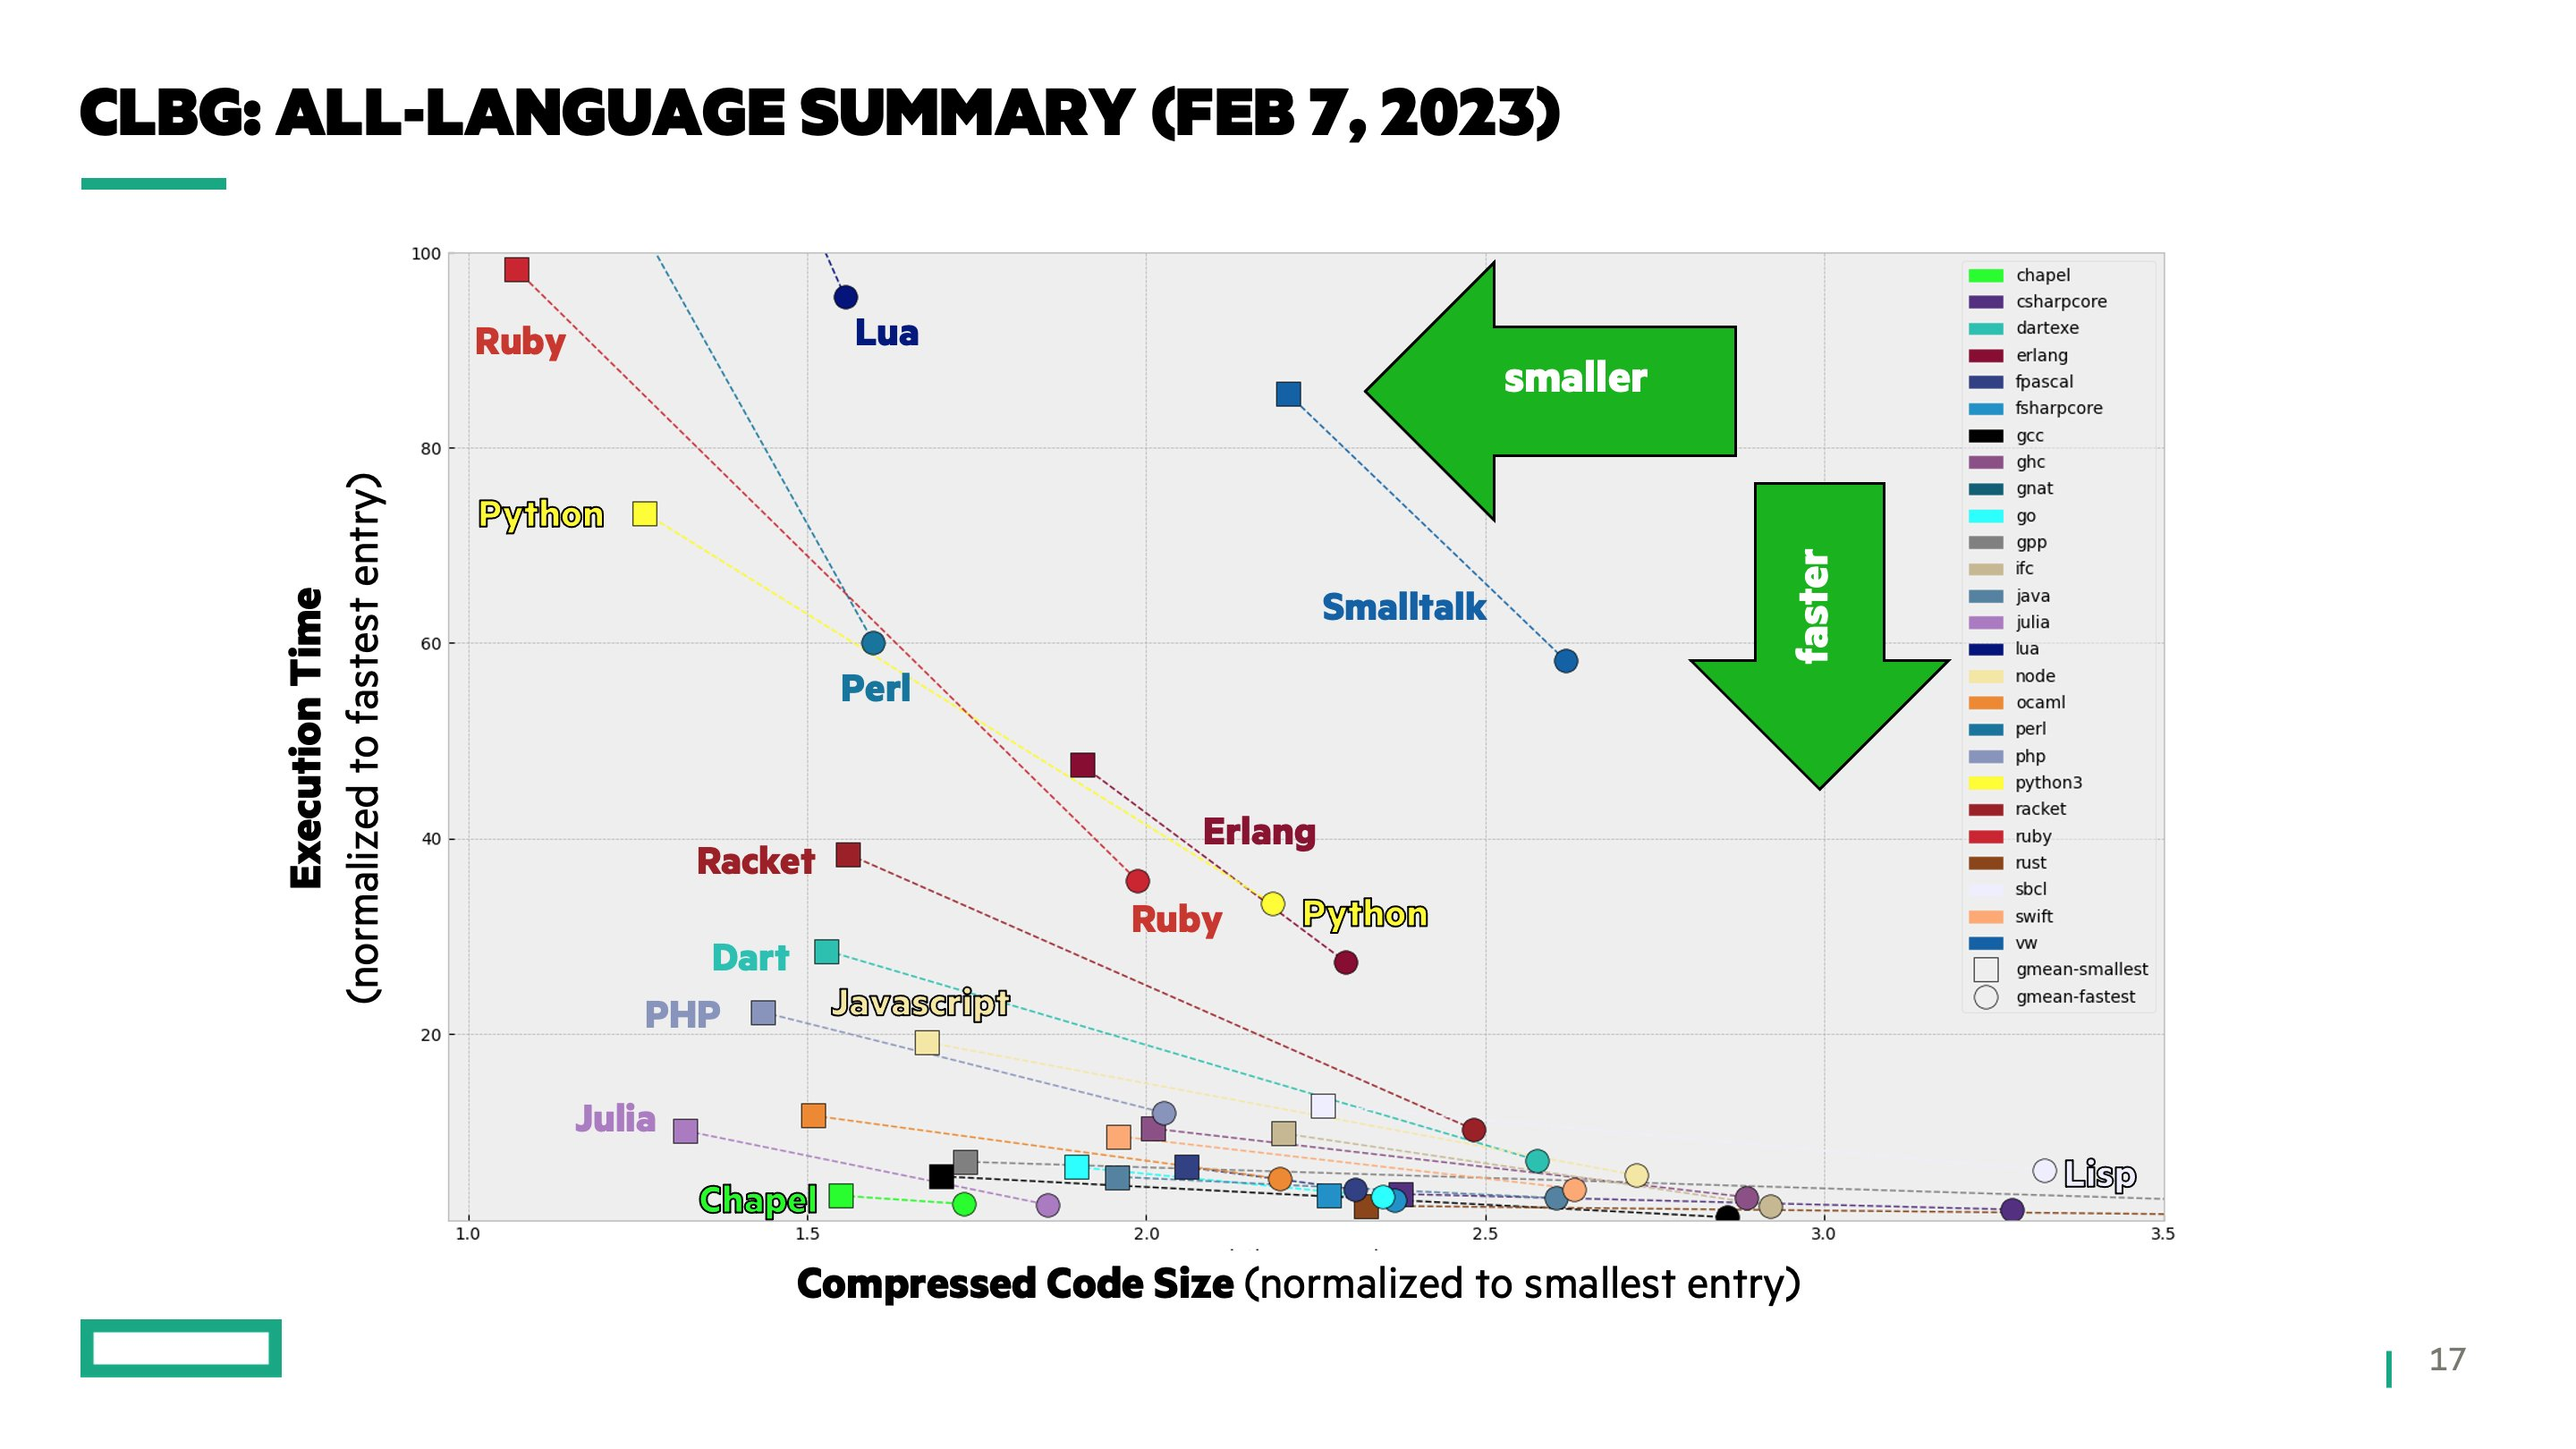
\includegraphics[width=0.45\textwidth]{speed_vs_codesize_comparison.jpeg}
        \caption{Micro-benchmarks, source: \url{https://julialang.org/benchmarks/}.}
        %Right: speed vs code size, source: devs of Chapel language.
        \label{fig:benchmarks}
    \end{figure}
\end{frame}

\begin{frame}
    \frametitle{Strong points -- Fluid coding}
    % TODO add omega\_pi ASCII code ?
    \begin{itemize}
        \item Unicode support, clear syntax
        \item Eliminates points of friction
        \begin{itemize}
            \item {\tt help?>}, {\tt @time}, {\tt @edit}
            \item Features-packed REPL
            \item Packages, environments : \texttt{juliaup}, \texttt{Pkg.jl}
        \end{itemize}
    \end{itemize}
\end{frame}

\begin{frame}
    \frametitle{Strong points -- Community}
    \begin{itemize}
        \item Online community: \url{https://discourse.julialang.org}
        \item 100k+ available libraries
        \item State-of-the art in: ODE, ML, \dots
    \end{itemize}
\end{frame}

\begin{frame}
    \frametitle{Strong points -- Community}
    \begin{figure}[htbp]
        \centering
        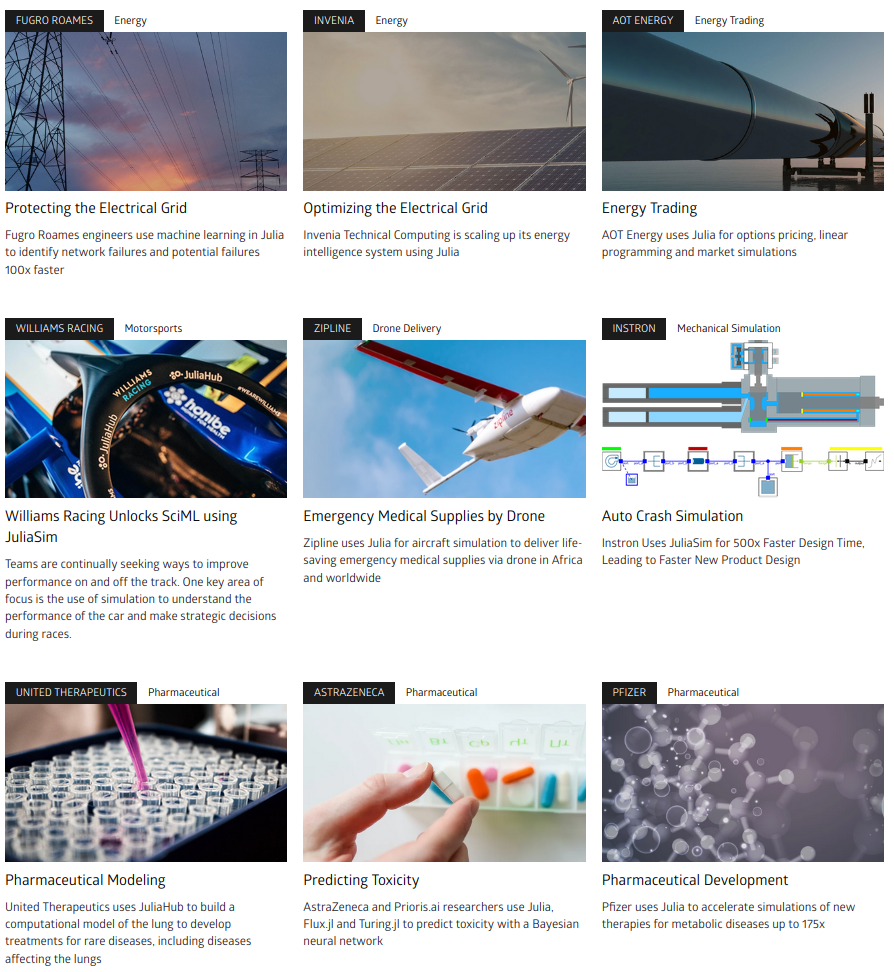
\includegraphics[width=0.45\textwidth]{julia_case_studies.png}
        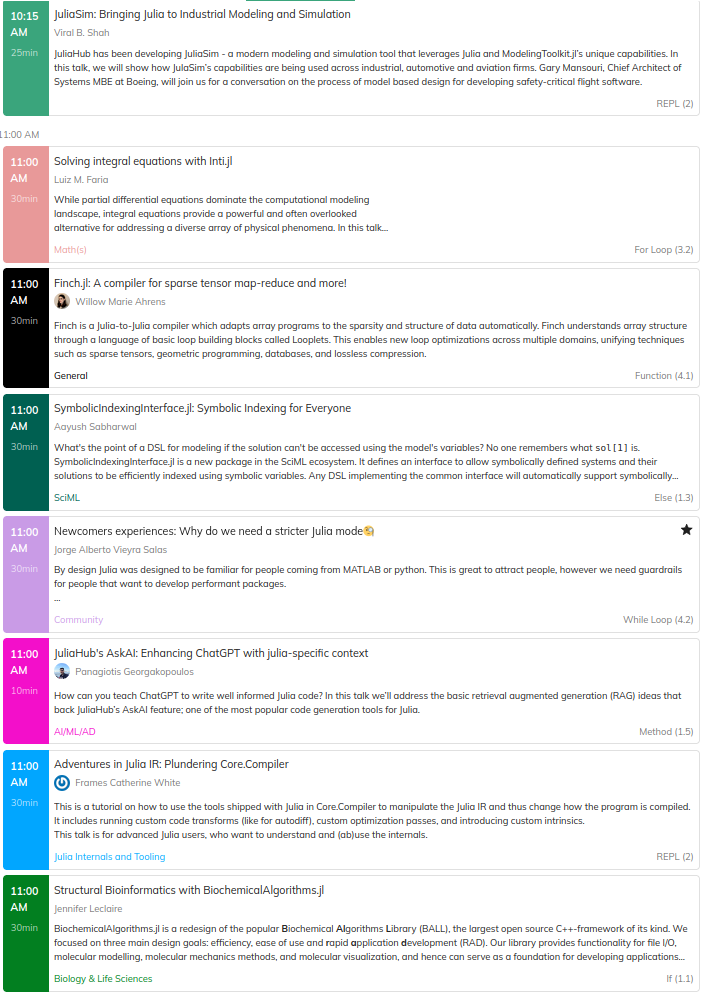
\includegraphics[width=0.35\textwidth]{juliacon_talks.png}
        \caption{Left: \url{https://info.juliahub.com/case-studies}. Right: JuliaCon 2024 talks, Wednesday morning.}
        \label{fig:julia_use}
    \end{figure}
\end{frame}


\begin{frame}
    \frametitle{Strong points -- Extensibility}
    % TODO add image: code C vs Julia
    \begin{itemize}
        \item Composability with other languages: {\tt ccall}, {\tt fcall}, {\tt pycall}, {\tt rcall}\dots
        \item Massive code re-use within Julia: multiple dispatch!
        \item Developing a package is easy (pkg creation, Julia written in Julia)
    \end{itemize}
\end{frame}

\begin{frame}
    \frametitle{Strong points -- Reproducibility}
    \begin{figure}[htbp]
        \centering
        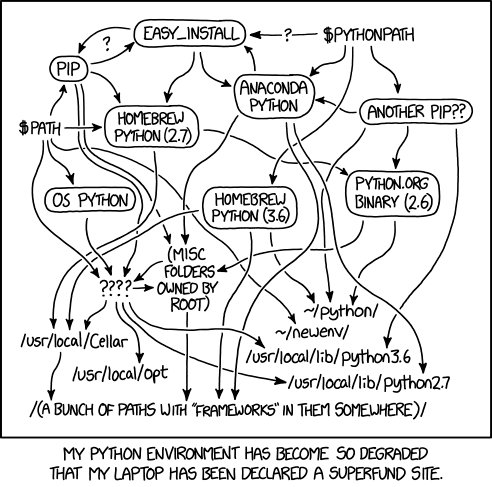
\includegraphics[width=0.4\textwidth]{python_environment.png}
        \caption{Python Environment (\url{https://xkcd.com/1987/})}
        \label{fig:xkcd_py_env}
    \end{figure}
    \pause
    \begin{itemize}
        \item Julia: {\tt juliaup}, {\tt Pkg.jl}, {\tt pkg>} mode\dots
        \item Readability
    \end{itemize}
\end{frame}

\section{[Interactive] optimizing Julia code}

\begin{frame}
    \frametitle{TO DO during interactive optimisation}
    \begin{itemize}
        \item Key points:
        \begin{itemize}
            \item Naive code can be very slow: follow simple rules !
            \item Optimize \textit{when you need to}
        \end{itemize}
        \pause
        \item Two critical points: type stability, and memory allocation!
        \item Secondary aspects: eg. encapsulating in functions
        \pause
        \item Cf. \footnotesize{\url{https://docs.julialang.org/en/v1/manual/performance-tips/}}
        \pause
        \item Tools!
        \begin{itemize}
            \item \texttt{@time} / BenchmarkTools.jl / Profiler or VS Code profiler
            \item \texttt{@code\_warntype} / JET.jl / Cthulhu.jl
            \item AllocationCheck.jl
        \end{itemize}
    \end{itemize}
\end{frame}

\begin{frame}
    \frametitle{Advanced Julia concepts}
    \begin{itemize}
        \item Just-in-time compilation
        \item Multiple dispatch
        \item Metaprogramming
        \item And much more!
    \end{itemize}
\end{frame}


\section{Conclusion}

\begin{frame}[plain, standout]
    Should you switch to Julia?
\end{frame}

\begin{frame}
    \frametitle{Comparing to other languages}
    \centering

    \begin{tabular}{m{2.5cm} | m{6cm}}
        Compared to\dots & Julia is \\ \hline
        Python\only<5->{*} & Faster, one language does it all \pause \\
        MATLAB & FOSS, easier, more general \pause \\
        C\only<5->{*} & Faster, quicker to write \pause \\
        TRIP & Released \emoji{upside-down-face}
    \end{tabular}
    \pause
    \vspace{10pt}

    *\small{You can even call these from Julia without overhead!}

\end{frame}


\begin{frame}
    \frametitle{Use Julia if...}
    \begin{itemize}
        \item You want to quickly write code
        \pause
        \item You want to write quick code
        \pause
        \item You want to use modern features and QOL
        \pause
        \item You value free and open-source software (FOSS)
        \pause
        \item You want to look cool \emoji{smiling-face-with-sunglasses}
    \end{itemize}
\end{frame}


\begin{frame}
    \frametitle{Caveats}
    \begin{itemize}
        \item 1.5 language problem
        \item Language is still evolving
        \item Can do some things I'm not fond of (general metaprogramming)
        \item Large compiled binaries
        \item Subpar static analysis
        \item Large memory consumption
    \end{itemize}
    % https://viralinstruction.com/posts/badjulia/
\end{frame}


\begin{frame}
    \frametitle{Why do \textit{I} use Julia?}
    \begin{itemize}
        \item Automatic differentiation
        \item Convinced by the advantages...
        \pause
        \item And can contribute to fixing the flaws!
    \end{itemize}
\end{frame}


\begin{frame}
    \frametitle{Resources -- some tools}
    \centering
    \begin{tabular}{| m{5cm} | m{5cm}|}
        \hline
        \makecell{\textbf{IDE}\\ REPL, {\tt Pluto.jl}, VS Code\dots}
        &
        \onslide<2->{\makecell{\textbf{Visualisation}\\ {\tt Makie.jl}, {\tt Plots.jl}\dots}}
        \\ \hline
        \onslide<3->{\makecell{\textbf{HPC}\\ {\tt Threads.jl},\\ {\tt Distributed.jl}, JuliaGPU\dots}}
        &
        \onslide<4->{\makecell{\textbf{Package dev}\\ {\tt Revise.jl}, \\{\tt PkgTemplates.jl} \dots}}
        \\
        \hline
    \end{tabular}
\end{frame}


\begin{frame}
    \frametitle{Resources -- useful links}
    \begin{itemize}
        \item MIT course: {\footnotesize \url{https://computationalthinking.mit.edu/Spring21/}}
        \item High-speed Julia: {\footnotesize \url{https://gdalle.github.io/JuliaPerf-CERMICS/}}
        \item Performance tips: {\footnotesize \url{https://docs.julialang.org/en/v1/manual/performance-tips/}} and its references
    \end{itemize}
\end{frame}


\begin{frame}
    \frametitle{Resources -- general}
    \begin{itemize}
        \item Discourse: \url{https://discourse.julialang.org}
        \item Slack/Zulip
        \item Docs: \url{https://docs.julialang.org/en/v1/}
    \end{itemize}
\end{frame}

\begin{frame}[allowframebreaks, noframenumbering, plain]
	\nocite{*}
	\printbibliography
\end{frame}


\begin{frame}[plain, standout]
	\begin{center}
		\huge{Thank you for listening!}

		\small{Any questions?}
	\end{center}
\end{frame}


\appendix

\begin{frame}[fragile]
    \frametitle{Multiple dispatch - C code}

\begin{minted}[breaklines,escapeinside=\%\%,mathescape=true, linenos, numbersep=3pt, gobble=0, frame=lines, fontsize=\small, framesep=2mm,
    bgcolor=CodeBG]{cpp}
class Pet {
    public:
        string name;
};
string meets(Pet a, Pet b) { return "FALLBACK"; }

void encounter(Pet a, Pet b) {
    string verb = meets(a, b);
    cout << a.name << " meets " << b.name
         << " and " << verb << endl;
}
\end{minted}

\end{frame}


\begin{frame}[fragile]
    \frametitle{Multiple dispatch - C code 2}

\begin{minted}[breaklines,escapeinside=\%\%,mathescape=true, linenos, numbersep=3pt, gobble=0, frame=lines, fontsize=\small, framesep=2mm,
    bgcolor=CodeBG]{cpp}
class Dog : public Pet {};
class Cat : public Pet {};

string meets(Dog a, Dog b){ return "sniffs"; }
string meets(Dog a, Cat b){ return "chases"; }
string meets(Cat a, Dog b){ return "hisses"; }
string meets(Cat a, Cat b){ return "slinks"; }
\end{minted}

\end{frame}

\begin{frame}[fragile]
    \frametitle{Multiple dispatch - C code 3}

\begin{minted}[breaklines,escapeinside=\%\%,mathescape=true, linenos, numbersep=3pt, gobble=0, frame=lines, fontsize=\small, framesep=2mm,
    bgcolor=CodeBG]{cpp}
int main() {
    Dog fido; fido.name = "Fido";
    Dog rex; rex.name = "Rex";
    Cat whiskers; whiskers.name = "Whiskers";
    Cat spots; spots.name = "Spots";

    encounter(fido, rex);
    encounter(fido, whiskers);
    encounter(whiskers, rex);
    encounter(whiskers, spots);

    return 0;
}
\end{minted}

\end{frame}


\begin{frame}[fragile]
    \frametitle{Multiple dispatch - Julia code}

\begin{minted}[breaklines,escapeinside=\%\%,mathescape=true, linenos, numbersep=3pt, gobble=0, frame=lines, fontsize=\small, framesep=2mm,
    bgcolor=CodeBG]{julia}
abstract type Pet end
struct Dog <: Pet; name::String end
struct Cat <: Pet; name::String end

function encounter(a::Pet, b::Pet)
    verb = meets(a, b)
    println("$(a.name) meets $(b.name) and $verb")
end

meets(a::Dog, b::Dog) = "sniffs"
meets(a::Dog, b::Cat) = "chases"
meets(a::Cat, b::Dog) = "hisses"
meets(a::Cat, b::Cat) = "slinks"
\end{minted}
\end{frame}


\begin{frame}[fragile]
    \frametitle{Multiple dispatch - Julia code 2}

\begin{minted}[breaklines,escapeinside=<>,mathescape=true, linenos, numbersep=3pt, gobble=0, frame=lines, fontsize=\small, framesep=2mm,
    bgcolor=CodeBG]{julia}
fido = Dog("Fido")
rex = Dog("Rex")
whiskers = Dog("Whiskers")
spots = Dog("Spots")

encounter(fido, rex)
encounter(fido, whiskers)
encounter(whiskers, rex)
encounter(whiskers, spots)
\end{minted}
\end{frame}

\begin{frame}
    \frametitle{Multiple dispatch - results}
    {\tt {\bf \$ julia pets.jl} \\
    Fido meets Rex and sniffs \\
    Fido meets Whiskers and chases \\
    Whiskers meets Rex and hisses \\
    Whiskers meets Spots and slinks \\ \\
    {\bf\$ clang++ pets.cxx -o pets \\
    \$ ./pets}\\
    Fido meets Rex and FALLBACK \\
    Fido meets Whiskers and FALLBACK \\
    Whiskers meets Rex and FALLBACK \\
    Whiskers meets Spots and FALLBACK
    }

    

\end{frame}


\end{document}